\section{Network, Data and Battery Models}
\label{ch1:sec:data-and-network-models}

All key network parameters and their associated cost functions have now been established.
In this section the network model and power flow simulation, from which all aforementioned key network parameters were extracted are explained.
Also, all data that is used throughout the presented research is included, too.

\subsection{Standardised Network Model}
\label{ch1:subsec:standardised-network-model}

The IEEE Power and Energy Society (IEEE-PES) provided several multi-node test feeder cases.
These test cases used to be limited to distribution networks in the United States.
In 2015 however, they published a standardised model of a LV distribution network for the UK power network.
This model is called the ``European Low Voltage Test Feeder'' and an OpenDSS compatible version can now be obtained from their website \cite{DistributionTestFeeders2017}.
Within the context of this work, this feeder is referred to as the ``LV Test Case'' and a network plot of this feeder has been included for reference.

\begin{figure}\centering
	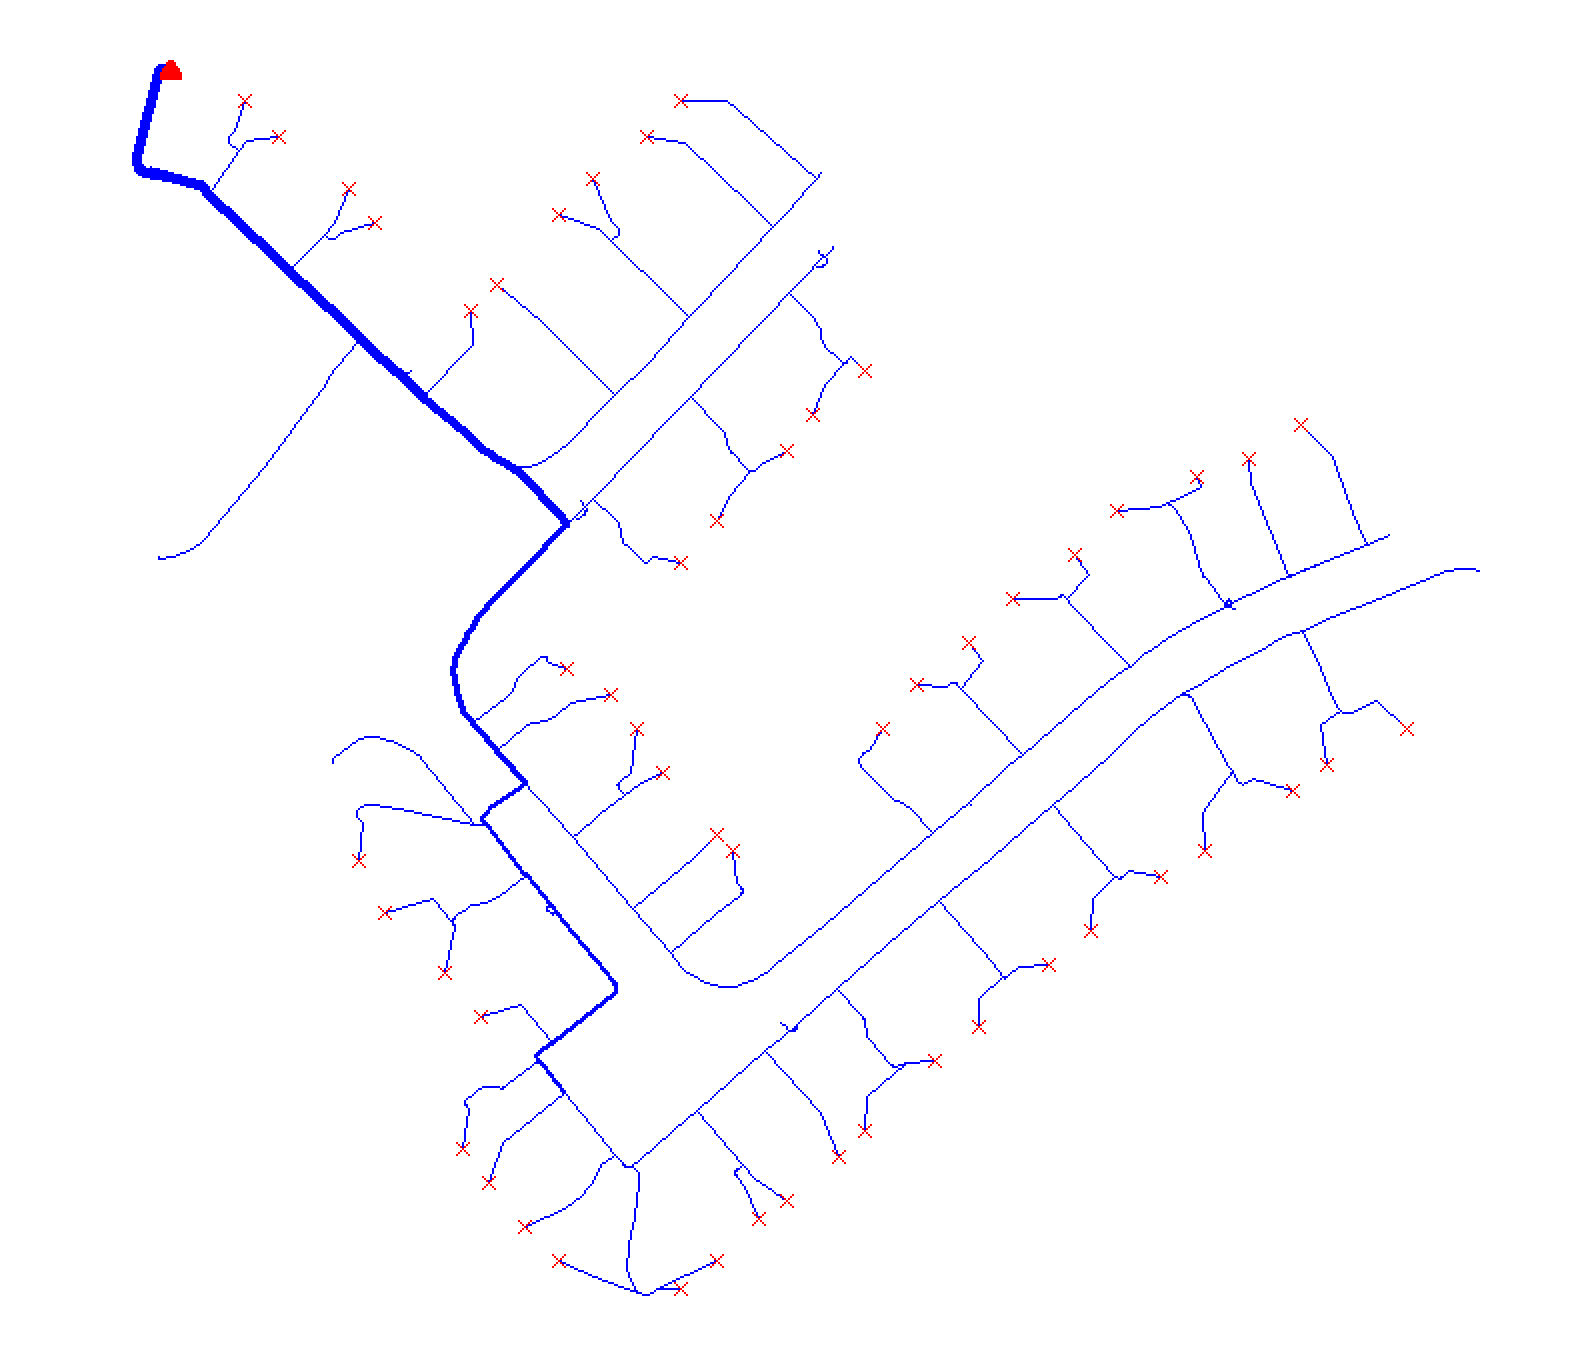
\includegraphics[width=0.8\textwidth]{_chapter1/fig/network-plot-LVTestCase}
	\caption{A power flow plot of the IEEE-PES European Test Case Feeder, i.e. a LV distribution network in the UK.}
	\label{ch1:fig:network-plot-LVTestCase}
\end{figure}

Here, a substation (triangle in north west) provides power to the feeder, and the power flowing through this feeder is visualised by the thickness of its lines.
In total, there are 55 single-phase households connected to the substation, which represents a medium-sized UK feeder.

\subsection{Load Profiles: Minutely and Half-Hourly}

Alongside the LV Test Case, 100 minutely demand profiles were supplied; each profile being 24h long.
Therefore, by assigning one load profile to each customer, a series of 1440 snapshot simulations could be run in OpenDSS in order to simulate the variation and volatility in demand over the entire day.
Since the provided power values only provided active power values, a standardised power factor of 0.95 was used for all loads to calculate their reactive component.
This non-unity power factor simulates a certain inductive load, which would otherwise be neglected.

\nomenclature{$s_\text{net}(t)$}{Apparent network load at time $t$ (Chapter \ref{ch1})}
\nomenclature{$s_{\text{load},i}(t)$}{Apparent load power for load $i$ at time $t$, where $s_{\text{load},i}(t) \in \textbf{s}_\text{load}(t)$ (Chapter \ref{ch1})}
\nomenclature{$\textbf{s}_\text{load}(t)$}{Apparent load power vector of all loads at time $t$ (Chapter \ref{ch1})}

Before any scheduling could take place, the total network load, $s_\text{net}(t)$, had to be calculated by aggregating all customer loads:

\begin{equation}
	s_\text{net}(t) := \sum_{i=1}^{I} s_{\text{load},i}(t)
	\text{ where } I \in \mathbb{Z}_{\geq 0}
\end{equation}

This demand is however at minutely resolution.
Computing the ESMU schedule at this resolution (or any sub-half-hourly resolution) for an entire day is very computationally demanding and highly ineffective.
Mainly, since cutting edge research in load forecasting has shown that demand variability due to behavioural unpredictability makes forecasting at high temporal resolution unfeasible, but also since traditional forecasts are generally provided at half-hourly resolution.
Therefore, the sub-half-hourly profile had to be down-sampled or extrapolated to a coarser resolution, by using a synchronisation function $k(t)$.
This function links the original sub-half-hourly to a resulting half-hourly time-series like so:

\begin{equation}
	k(t) := \left\lfloor\frac{t-1}{K\Delta t}\right\rfloor+1
	\label{ch1:equ:synchronisation-function}
\end{equation}

\nomenclature{$\Delta t$}{High resolution sample period, i.e. sub-half hourly or minutely, where $\Delta t \in \mathbb{Z}^{>0}$ (Chapter \ref{ch1})}
\nomenclature{$K$}{Number of blocks to downsample the sub-half-hourly profile into, where $K \in \mathbb{Z}^{>0}$ and $\frac{T_\text{sch}}{K} \in \mathbb{Z}^{>0}$ (Chapter \ref{ch1})}
\nomenclature{$k(t)$}{Synchronisation function used to downsample the sub-half-hourly profile (Chapter \ref{ch1})}
\nomenclature{$k$}{Half-hourly timing, where $k \in [1, \dots, K]$ (Chapter \ref{ch1})}
\nomenclature{$T_\text{sch}$}{Scheduling horizon, where $T_\text{sch} \in \mathbb{Z}^{>0}$ (Chapter \ref{ch1})}

Here, $\Delta t$ is the sampling period (i.e. minutely period) of the simulation, and $K$ is number of low-resolution blocks.
It should be noted that the integer multiple of $K$ has to equate to the scheduling horizon's length, $T_\text{sch}$; i.e. $T_\text{sch} \overset{!}{=} \alpha K \text{ where } \alpha \in \mathbb{Z}^{>0}$.
Only in this case can the sub-half-hourly profile be divided into a complete set of chunks, where each chunk is of length $K\Delta t$.
Therefore, the resulting half-hourly network load, $s^{*}_\text{net}(t)$, can be defined as follows:

\begin{equation}
	s^*_{network\;\;load}(t^*) = \frac{T^*}{T}\sum_{t=1}^{\frac{T}{T^*}}s_{network\;\;load}\left(\frac{T}{T^*}(t^*-1) + t\right) \forall t^* \text{ where } t^* \in [1, \dots, T^{*}]
	\label{ch1:equ:down-sampling-to-half-hourly}
\end{equation}

Since all power values from a period of $k(t)K \rightarrow (k(t)+1)K-1$ are equal, a simplified half-hourly power vector is introduced as $p_\text{net}(k)$. 
In this and any subsequent vector, half-hourly timing is indicated by using the half-hourly time $k$ instead of the sub-half-hourly time $t$, where $k \in [1, \dots, K]$ and $K \in \mathbb{Z}^{>0}$.
The link between $s^{*}_\text{net}(t)$ and $s_\text{net}(k)$ is therefore defined as:

\begin{equation}
	s_\text{net}(k) := s^{*}_\text{net}(Kk) \forall k
	\label{ch1:equ:half-hourly-power-profile}
\end{equation}

It is worth mentioning, that from here on all subsequent cost functions (i.e. any $\zeta$) that deal with half-hourly profiles, are functions that use the half-hourly timing $k$, whilst sub-half-hourly or real-time costs use the high-resolution timing $t$.
This difference will become important when differentiating between scheduling costs and the aforementioned network costs (which are based on a set of key network parameters).
Nonetheless, to illustrate how the original sub-half-hourly network load is extrapolated into the resulting half-hourly demand, both profiles are plotted in a figure below.

\begin{figure}\centering
	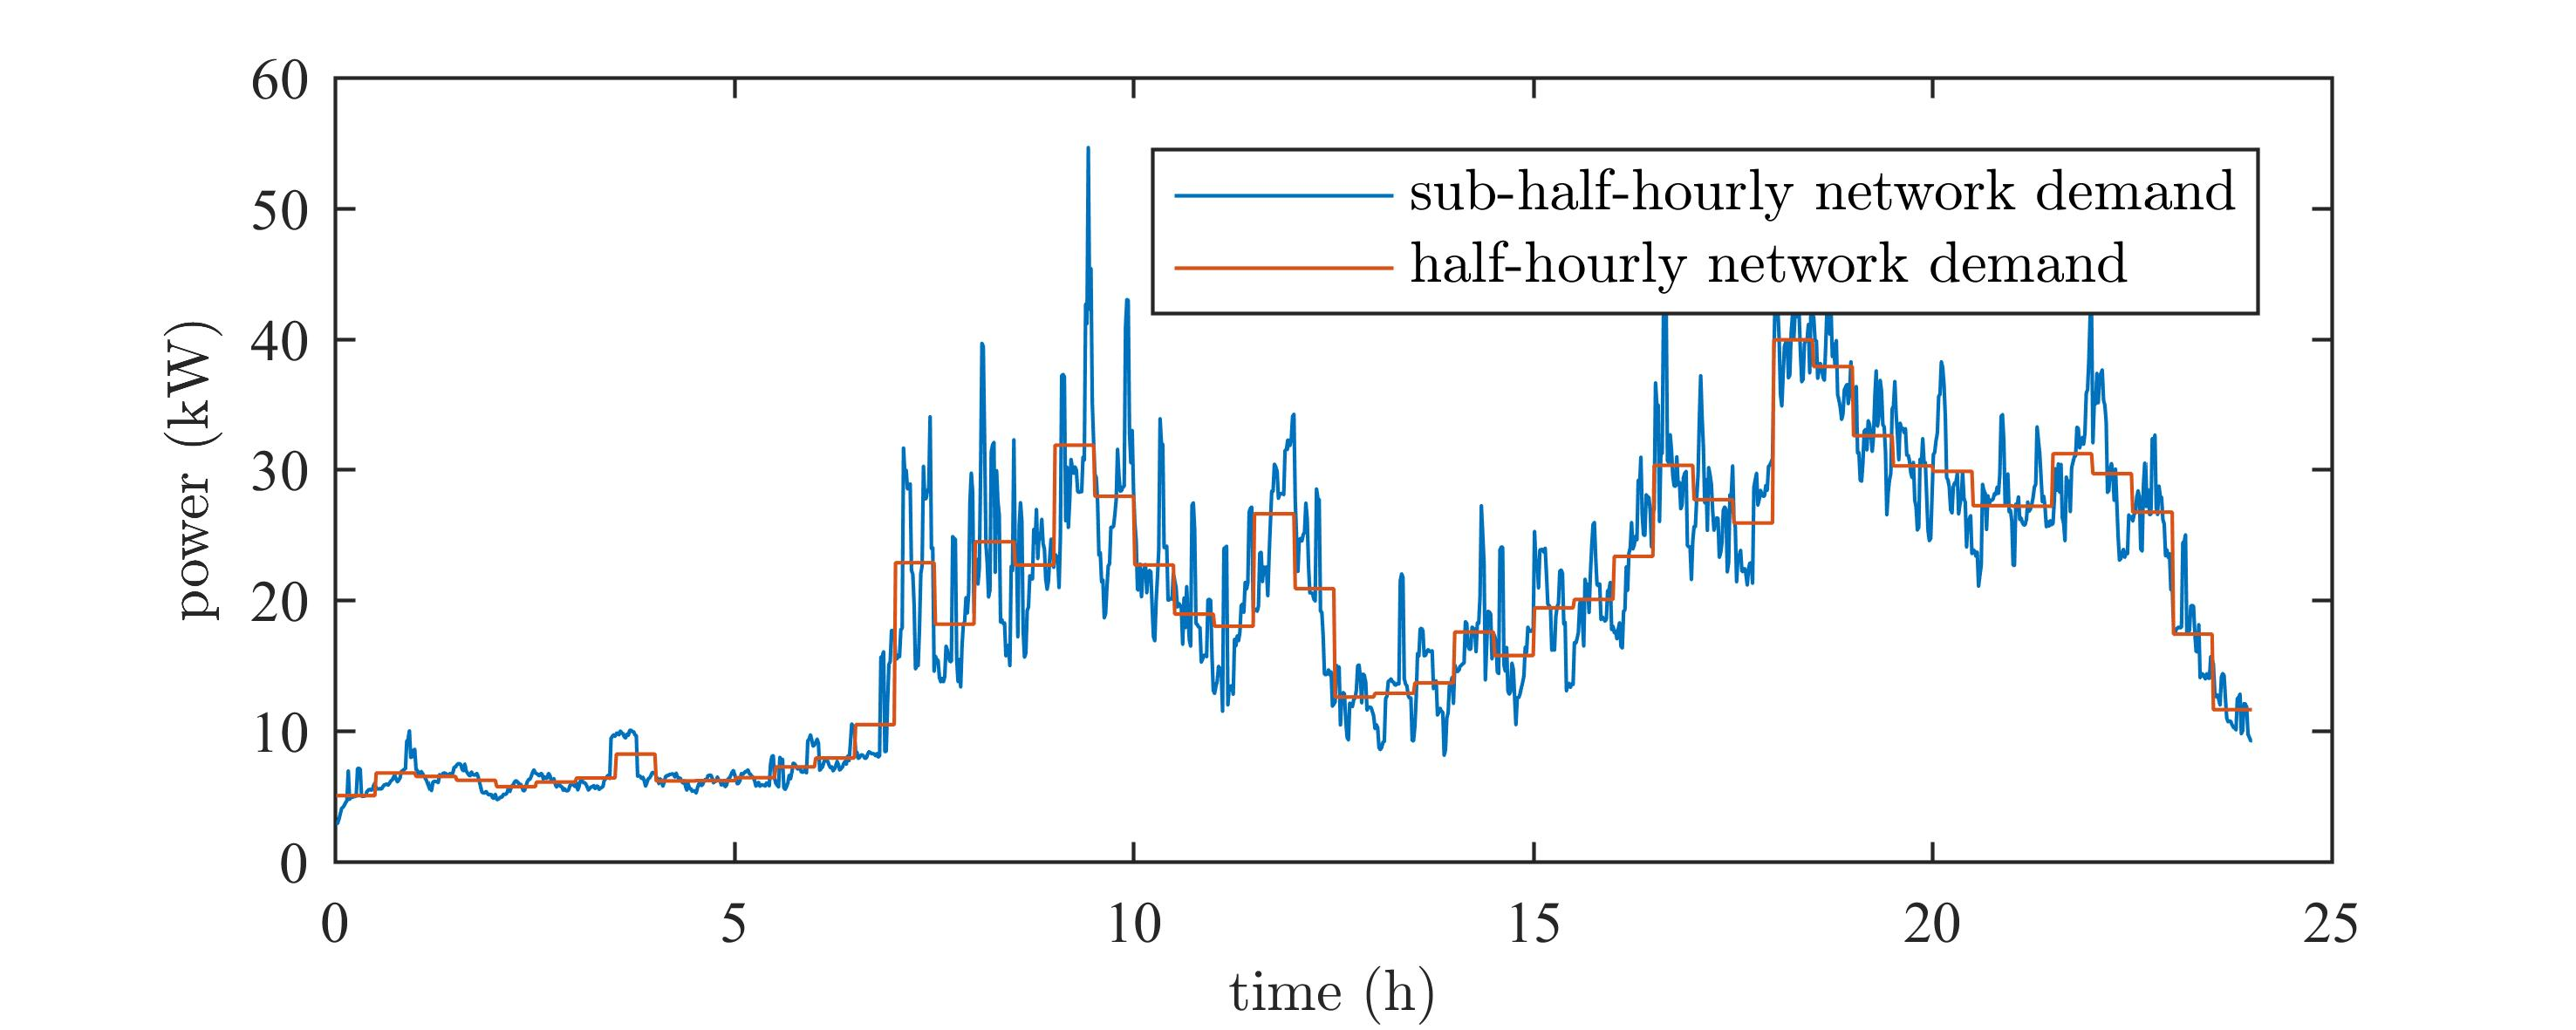
\includegraphics{_chapter1/fig/sub-half-horuly-demand-comparison}
	\caption{Highly variable and volatile demand profile vs half-hourly demand (i.e. a forecast under perfect foresight conditions)}
	\label{ch1:fig:sub-half-horuly-demand-comparison}
\end{figure}

In Figure \ref{ch1:fig:sub-half-horuly-demand-comparison}, it can be observed how the high variability and volatility in power is removed in the half-hourly profile.
When generating the ESMU schedules (which is addressed in Section \ref{ch1:subsec:esmu-schedule-generation}) these variations are neglected and the unwanted peak power demands are hence no longer sufficiently compensated.

\subsection{Battery Model}

\nomenclature{$S_\text{rating}$}{Rating of battery's power electronics, where $S_\text{rating} \in \mathbb{R}^{>0}$ (Chapter \ref{ch1})}

The ESMU systems that were deployed throughout the NTVV project consisted of two parts: the Power Management Unit (PMU) and the Energy Storage Unit (ESU).
The PMU controls the three-phase powers and links the ESU to the grid.
Each PMU's per phase power rating, $S_\text{rating}$, is 12kVA and, beside battery charging and discharging, can also perform filtering functions, e.g. compensating for harmonic distortion, reactive power and phase unbalance.
The ESU is a modular container of 12.5kWh of Li-Ion energy storage that can be aggregated to increase the total energy storage capacity.
All battery monitoring, conditioning and regulation is performed within the ESU and hence need not be considered for the scope of this work.
However, control instructions that are sent to the ESMU system should not request the device to operate outside its own specifications, i.e. under- or over-charge the batteries.

In order to simulate this ESMU system and its energy storing behaviour, a model is developed from the given device specifications.
This model includes both an charge-discharge efficiency and standby losses.
The charge-discharge efficiency is related to the efficiency of the PMU's power converters, which are quoted to have a round trip efficiency of 98\%.
The standby losses on the other hand are associated to the nominal power drawn by the battery's control system as well as the battery's self-discharge rate.
It became common practice to assess the energy storage's charge level as the State of Charge (SOC) instead of using the actual charge stored.
This SOC is defined as:

\begin{equation}
	SOC(t) := \frac{E_{battery}(t)}{C_{battery}} \forall t
	\label{ch1:equ:state-of-charge-definition}
\end{equation}

\nomenclature{$C_\text{bat}$}{Battery capacity, where $C_\text{bat} \in \mathbb{R}^{>0}$ (Chapter \ref{ch1})}
\nomenclature{$E_\text{bat}(t)$}{Energy stored in battery at time $t$, where $E_\text{bat}(t) \in \mathbb{R}^{>0}$ (Chapter \ref{ch1})}
\nomenclature{$\eta$}{Round-trip efficiency of power electronics, where $\eta \in (0, 1]$ (Chapter \ref{ch1})}
\nomenclature{$s_{\text{bat},\phi}(t)$}{Single-phase apparent battery power for phase $\phi$ at time $t$, where $s_{\text{bat},\phi}(t) \in \textbf{s}_\text{bat}(t)$ (Chapter \ref{ch1})}
\nomenclature{$s_{\text{ESMU},\phi}(t)$}{Single-phase apparent ESMU power for phase $\phi$ at time $t$, where $s_{\text{ESMU},\phi}(t) \in \textbf{s}_\text{ESMU}(t)$ (Chapter \ref{ch1})}


SOC is therefore defined for any given time $t$, as the actual energy stored in the ESU, $E_\text{bat}(t)$, divided by the total capacity of the system, $C_\text{bat}$.
With the conversion efficiency as the factor $\eta$, the battery charge and discharge power, $s_\text{bat}(t)$ (in kW)\footnote[1]{It is worth mentioning, that $s$ is chosen for apparent power (i.e. active and reactive power in kVA), yet $s_\text{bat}$ is purely active (i.e. in kW).}, can be calculated for any given ESMU power, $\textbf{s}_\text{ESMU}(t)$ (where $s_{\text{ESMU},\phi}(t) \in \textbf{s}_\text{ESMU}(t)$).

\begin{equation}
\begin{split}
	s_\text{bat}(t) = 
	\begin{cases}
		\eta\text{Re}\left\{\sum_{\phi=1}^{\Phi}s_{\text{ESMU},\phi}(t)\right\} &\text{ if } \text{Re}\left\{\sum_{\phi=1}^{\Phi}s_{\text{ESMU},\phi}(t)\right\} \geq 0\\
		\frac{1}{\eta}\text{Re}\left\{\sum_{\phi=1}^{\Phi}s_{\text{ESMU},\phi}(t)\right\} &\text{ otherwise}
	\end{cases} \forall t \\
	\text{and } \phi \in [1, \dots, \Phi] \text{ and } \Phi \in \mathbb{Z}^{>0}
\end{split}
\label{ch1:equ:battery-power-definition}
\end{equation}

\nomenclature{$C_f$}{Charge factor or ``C-factor'' of the battery, where $C_f \in \mathbb{R}^{>0}$ (Chapter \ref{ch1})}

Although the ESMU's PSU rating, $S_\text{rating}$, may allow for a maximum power consumption of 36kVA (i.e. $=3\times12\text{kVA}$), the charging power is internally limited, due to a charging factor, $C_f$, which was chosen to be the standard value of 1.6.
This factor is the ratio between the battery's maximum discharge power and its total capacity (i.e. $s_\text{bat}(t) \leq C_f \cdot C_\text{bat} \forall t$).
Assuming that this charge/discharge power is applied and remains constant during a sample period of $\Delta t$, an equation describing the change in stored energy can be formulated.

\begin{equation}
	\Delta E_{battery}(t) = s_{battery}(t)t_s \forall t
	\label{ch1:equ:change-in-energy}
\end{equation}

\nomenclature{$\mu$}{Self-discharge losses of battery, where $\mu \in (0, 1]$ (Chapter \ref{ch1})}
\nomenclature{$\Delta E_\text{bat}(t)$}{Change in stored energy at time $t$ (Chapter \ref{ch1})}
\nomenclature{$SOC(t)$}{State of charge at time $t$ (Chapter \ref{ch1})}

As already mentioned, the energy level is however affected by standby losses, which are captured by a self-discharge factor, $\mu$.
Therefore, when adding the change in energy level to the current energy level in order to calculate the next energy level, this factor needs to be taken into account.

\begin{equation}
	E_{battery}(t+1) = \mu\left(\Delta E_{battery}(t) + E_{battery}(t)\right)
\label{ch1:equ:next-energy}
\end{equation}

In an ideal case, $\mu = 1$, where no energy would be lost in the storage system.
Finally, by adding the current energy level to the change in energy level, and by substituting Equation \ref{ch1:equ:state-of-charge-definition}, the next SOC can be found:

\begin{equation}
	SOC(t+\Delta t) := \mu\left(\frac{p_\text{bat}(t)\Delta t}{C_\text{bat}} + SOC(t)\right)
	\label{ch1:equ:next-state-of-charge}
\end{equation}

When summarising $\hat{s}_\text{ESMU}(t) = \text{Re}\left\{\sum_{\phi=1}^{\Phi}s_{\text{ESMU},\phi}(t)\right\}$ and substituting Equation \ref{ch1:equ:battery-power-definition} into Equation \ref{ch1:equ:next-state-of-charge}, then $SOC(t+\Delta t)$ can be rewritten as:

\begin{equation}
	SOC(t+\Delta t) := 
	\begin{cases}
		\mu\left(\frac{\eta \hat{s}_\text{ESMU}(t)\Delta t}{C_\text{bat}} + SOC(t)\right)	&\text{if } \hat{s}_\text{ESMU}(t) \geq 0\\
		\mu\left(\frac{\hat{s}_\text{ESMU}(t)\Delta t}{\eta C_\text{bat}} + SOC(t)\right) &\text{otherwise}
	\end{cases}
	\forall t
	\label{ch1:equ:next-state-of-charge-2}
\end{equation}

A flowchart to visually capture the model, as it is explained from Equation \ref{ch1:equ:state-of-charge-definition} to \ref{ch1:equ:next-state-of-charge}, is presented below.

\begin{figure}\centering
% Define some block styles
\tikzstyle{input} = [%
	draw,%
	ellipse,%
	fill=green!20,%
	minimum height=2em,%
]
\tikzstyle{result} = [%
	draw,%
	ellipse,%
	fill=blue!20,%
	minimum height=2em,%
]
\tikzstyle{output} = [%
	draw,%
	ellipse,%
	fill=yellow!20,%
	minimum height=2em,%
]
\tikzstyle{decision} = [%
	diamond,%
	draw,%
	text width=4.5em,%
	text badly centered,%
	inner sep=0pt%
]
\begin{tikzpicture}[node distance=3cm, shorten >= 1pt, >=stealth', auto]

	% Define nodes
    \node (power_esmu) [input] {$\textbf{s}_{ESMU}(t)$};
    \node (is_charging) [decision, right of=power_esmu] {charging\footnotemark[2]};
    \node (charging) [state, above right of=is_charging] {$\times\eta$};
    \node (discharging) [state, below right of=is_charging] {$\times\frac{1}{\eta}$};
    \node (power_battery) [result, below right of=charging] {$s_{battery}(t)$};
    \node (sample) [state, right of=power_battery] {$\times \tau$};
    \node (change_energy_battery) [result, below of=sample, yshift=5mm] {$\Delta E_{battery}(t)$};
    \node (add) [state, below of=change_energy_battery, yshift=5mm] {$+$};
    \node (current_energy_battery) [result, left of=add] {$E_{battery}(t)$};
    \node (multiply) [state, left of=current_energy_battery] {$\times C_{battery}$};
    \node (current_soc) [input, left of=multiply] {$SOC(t)$};
    \node (losses) [state, below of=add, yshift=5mm] {$\times \mu \tau$};
	\node (next_energy) [result, left of=losses, xshift=-5mm] {$E_{battery}(t+1)$};
	\node (divide) [state, left of=next_energy, xshift=-5mm] {$\div C_{battery}$};
	\node (next_soc) [output, left of=divide, xshift=-5mm] {$SOC(t+1)$};

	% Draw lines
	\draw [->] (power_esmu) to (is_charging);
	\draw [->, bend left] (is_charging) to node {yes} (charging);
	\draw [->, bend right] (is_charging) to node [swap] {no} (discharging);
	\draw [->, bend left] (charging) to (power_battery);
	\draw [->, bend right] (discharging) to (power_battery);
	\draw [->] (power_battery) to (sample);
	\draw [->] (sample) to (change_energy_battery);
	\draw [->] (change_energy_battery) to (add);
	\draw [->] (current_soc) to (multiply);
	\draw [->] (multiply) to (current_energy_battery);
	\draw [->] (current_energy_battery) to (add);
	\draw [->] (add) to (losses);
	\draw [->] (losses) to (next_energy);
	\draw [->] (next_energy) to (divide);
	\draw [->] (divide) to (next_soc);
	
\end{tikzpicture}
\caption{Flowchart to calculate the next SOC (i.e. $SOC(t+1)$) based on current ESMU power (i.e. $\textbf{s}_{ESMU}(t)$) and current SOC (i.e. $SOC(t)$)}
\end{figure}

\footnotetext[2]{In the flowchart ``charging'' implies that $\sum_{\phi=1}^{\Phi}s_{ESMU,\phi}(t) \geq 0$ as explained in Equation \ref{ch1:equ:battery-power-definition}.}

Here, all green and blue fields indicate, respectively, model inputs and results.
The white states represent operations applied onto those inputs and results and in the end yield the output, i.e. the yellow field.
